\chapter{Electronic Design}

\graphicspath{{./Figures/Electronic Design/}}
% Overview of the chapter's focus.
In this chapter, the details of the electronic design are presented.
Where it emphasizes the details of the components' technical specifications and the selection process.
The chapter also discusses the circuit design and the PCB design.
In addition, the chapter discusses the power management and the power distribution.

% Emphasize the importance of electronic design in the context of the overall project.
The electronic design serves as a critical link between the robitic conceptual framework and the physical implementation of the robot.The electronic design translates the abstract control algorithm into tangible action and responses.
The electronic design directly influences the performance, responsiveness, adaptability to various scenarios.
\newpage

\section{Design Objectives and Constraints}
% Clearly define the objectives and goals for the electronic design
The main objectives of the electronic Design are to connect the different components and enable them to perform the desired tasks.
The electronic design is responsible for controlling the motors.
Robust communication between the electronic components is needed to ensure reliable operation of the robot.
% Discuss any constraints such as power requirements, size limitations.
The electronic design is constrained by the power requirements of the motors.
The motors require a high current to operate, and the electronic design should be able to provide the required current.
In addition, the electronic design is constrained by the size of the components and their placement in the robot body.

\section{Component Selection}
The component diagram is shown in a figure \ref{fig:componentsdiagram}shows the different components and their relationship with each other.
The main components are the microcontroller, rassberry pi, the motors, Distance sensor, Camera, the battery. The motors are chosen based on the calculations done in the mechanical design chapter. The microcontroller is chosen based on the complixity of the control algorithm and the processing power needed to run the control algorithm.

%figure of the components digram
\begin{figure}[h]
	\centering
	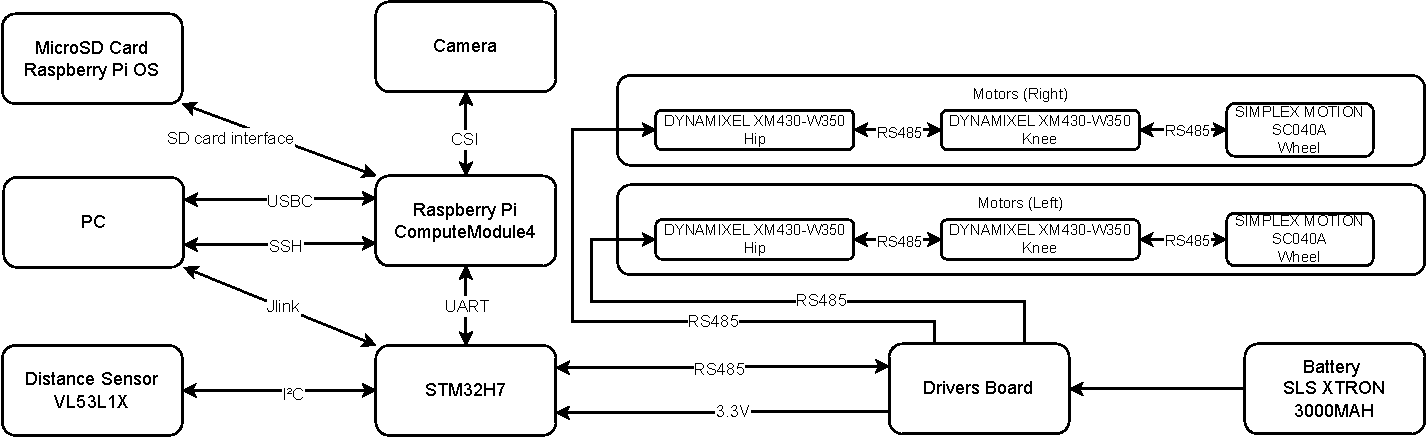
\includegraphics[width=1\linewidth]{Component_Diagram}
	%\includegraphics[width=0.5\linewidth]{Figures/Mechanical Design/Conceptual_Design}
	\caption[Components Diagram]{Components Diagram and there realationship with each other}
	\label{fig:componentsdiagram}
\end{figure}
\subsection{Hip and Knee Motors}
%Details the selection process for key electronic components like microcontrollers,sensors, actuators, power supplies, etc.
The DYNAMIXEL XM430-W350 is chosen as a motor for the hip joint and the knee joint. The motor is chosen because it has a high torque to weight ratio and it has a high resolution of 4096 steps per revolution. The motor has a built-in driver and it can be controlled using a serial communication protocol. The motor has a built-in encoder that can be used to measure the position of the motor. The motor has a maximum torque of 3.5 Nm and a maximum speed of 46 RPM. The motor has a maximum current of 2.1 A and a maximum voltage of 12 V. The motor has a weight of 82 g and a size of 28.5 x 46.5 x 34 mm.
%figure of the DYNAMIXEL XM430-W350 motor
\begin{figure}[h]
	\centering
	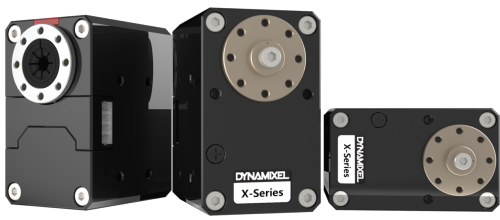
\includegraphics[width=0.5\linewidth]{DYNAMIXEL_XM430-W350}
	%\includegraphics[width=0.5\linewidth]{Figures/Mechanical Design/Conceptual_Design}
	\caption[DYNAMIXEL XM430-W350]{DYNAMIXEL XM430-W350}
	\label{fig:DYNAMIXEL_XM430-W350}
\end{figure}
%the
%from the info on the website for SIMPLEX MOTION SC040A
%Continuous output of 120W and 280 mNm torque at 4000rpm
%Brushless outer rotor motor with peak torque of 800 mNm
%Integrated drive electronics with 4096 positions/revolution position sensor
%PID regulator for position or speed control with torque limit
%Ramp control of speed or position
%Protection features for current, torque, voltage and temperature
%Serial interface RS485 with Modbus RTU protocol
%CANOpen 301 interface
%Quadrature encoder input for application use
%Interface signals for step motor emulation (step/direction)
%Up to 8 digital inputs and 4 analog inputs
%4 digital outputs capable of 30V/1A, with pulse, PWM and RC Servo control modes.
%PC based software for setup and testing
%subsection{Wheel Motors}
\subsection{Wheel Motors}
The SIMPLEX MOTION SC040A is chosen as a motor for the wheels. The motor is chosen since it has a output of 120W and 280 mNm torque at 4000rpm. The motor has a built-in driver and it can be controlled using RS485 serial communication protocol. The motor has  position and speed control with torque limit. The motor has a maximum torque of 800 mNm.
%figure of the SIMPLEX MOTION SC040A motor
\begin{figure}[h]
	\centering
	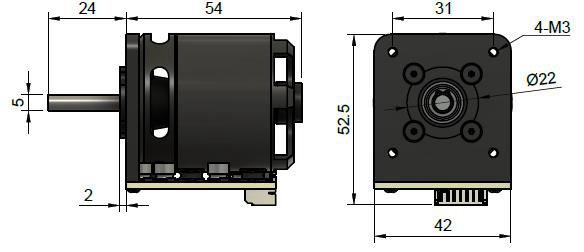
\includegraphics[width=0.5\linewidth]{SIMPLEX_MOTION_SC040A}
	%\includegraphics[width=0.5\linewidth]{Figures/Mechanical Design/Conceptual_Design}
	\caption[SIMPLEX MOTION SC040A]{SIMPLEX MOTION SC040A}
	\label{fig:SIMPLEX_MOTION_SC040A}
\end{figure}


%Rationale behind the choice of each component, focusing on specifications and performance requirements.

\subsection{Raspberry Pi}
The Raspberry Pi 4 compute module is chosen since it offers several advantages such as remote ssh connection via wifi. It can directly pass new control parameters to the microcontroller. It can be used to stream the video from the camera. The Raspberry Pi 4 compute module has a 64-bit quad-core ARM Cortex-A72 processor running at 1.5 GHz. It has 4 GB of LPDDR4-3200 SDRAM. The Raspberry Pi 4 compute module has a 32 GB eMMC Flash memory, a maximum current of 3 A and maximum voltage of 5.1 V.

%figure of the Raspberry Pi 4 compute module
\begin{figure}[h]
	\centering
	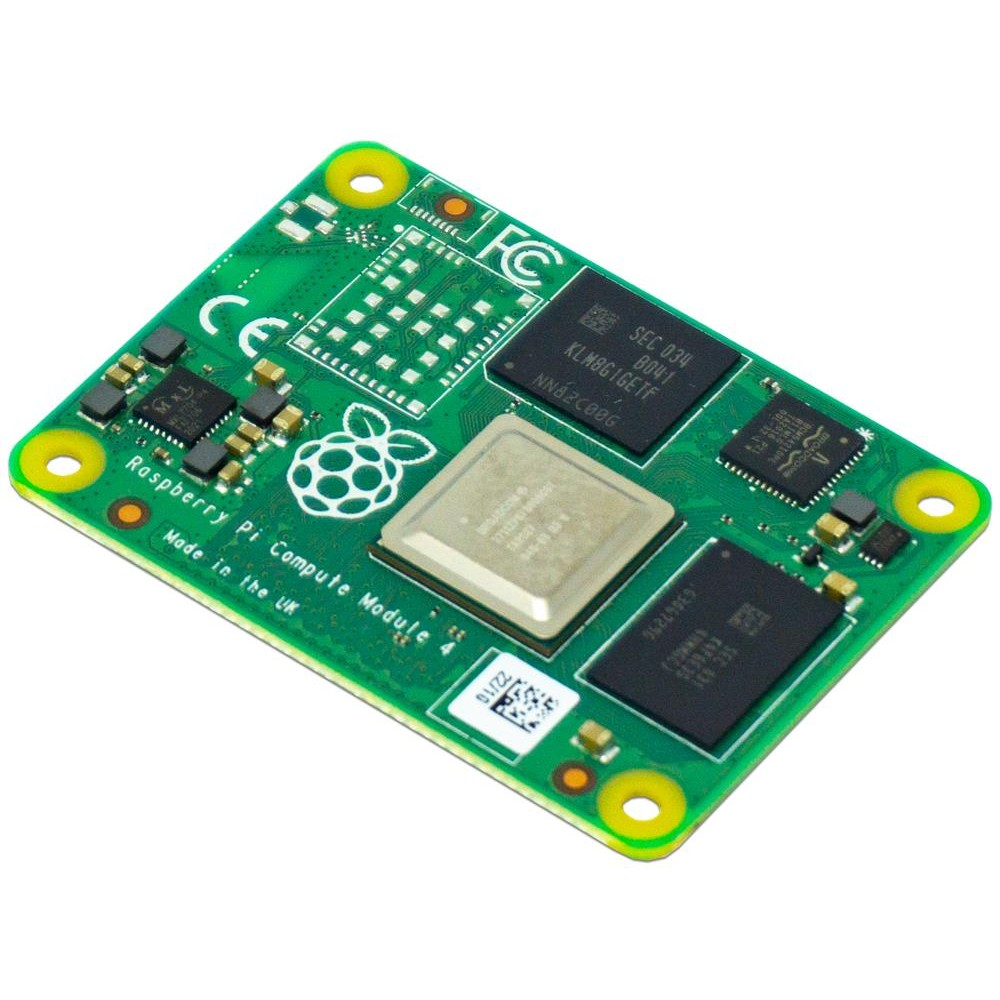
\includegraphics[width=0.5\linewidth]{Raspberry_Pi_4_compute_module}
	%\includegraphics[width=0.5\linewidth]{Figures/Mechanical Design/Conceptual_Design}
	\caption[Raspberry Pi 4 compute module]{Raspberry Pi 4 compute module}
	\label{fig:Raspberry_Pi_4}
\end{figure}
\newpage
\subsection{Distance Sensor}
The VL53L1X is chosen as a distance sensor for the robot. The sensor is chosen because it has a high accuracy and it has a high range. The sensor has a maximum range of 4 m. The sensor has a maximum accuracy of 1 mm. The sensor has a maximum field of view of 27 degrees. The sensor has a maximum current of 20 mA. The sensor has a maximum voltage of 3.6 V. The sensor has a weight of 1.6 g and a size of 4.4 x 2.4 x 1.0 mm.
%figure of the VL53L1X sensor
\begin{figure}[h]
	\centering
	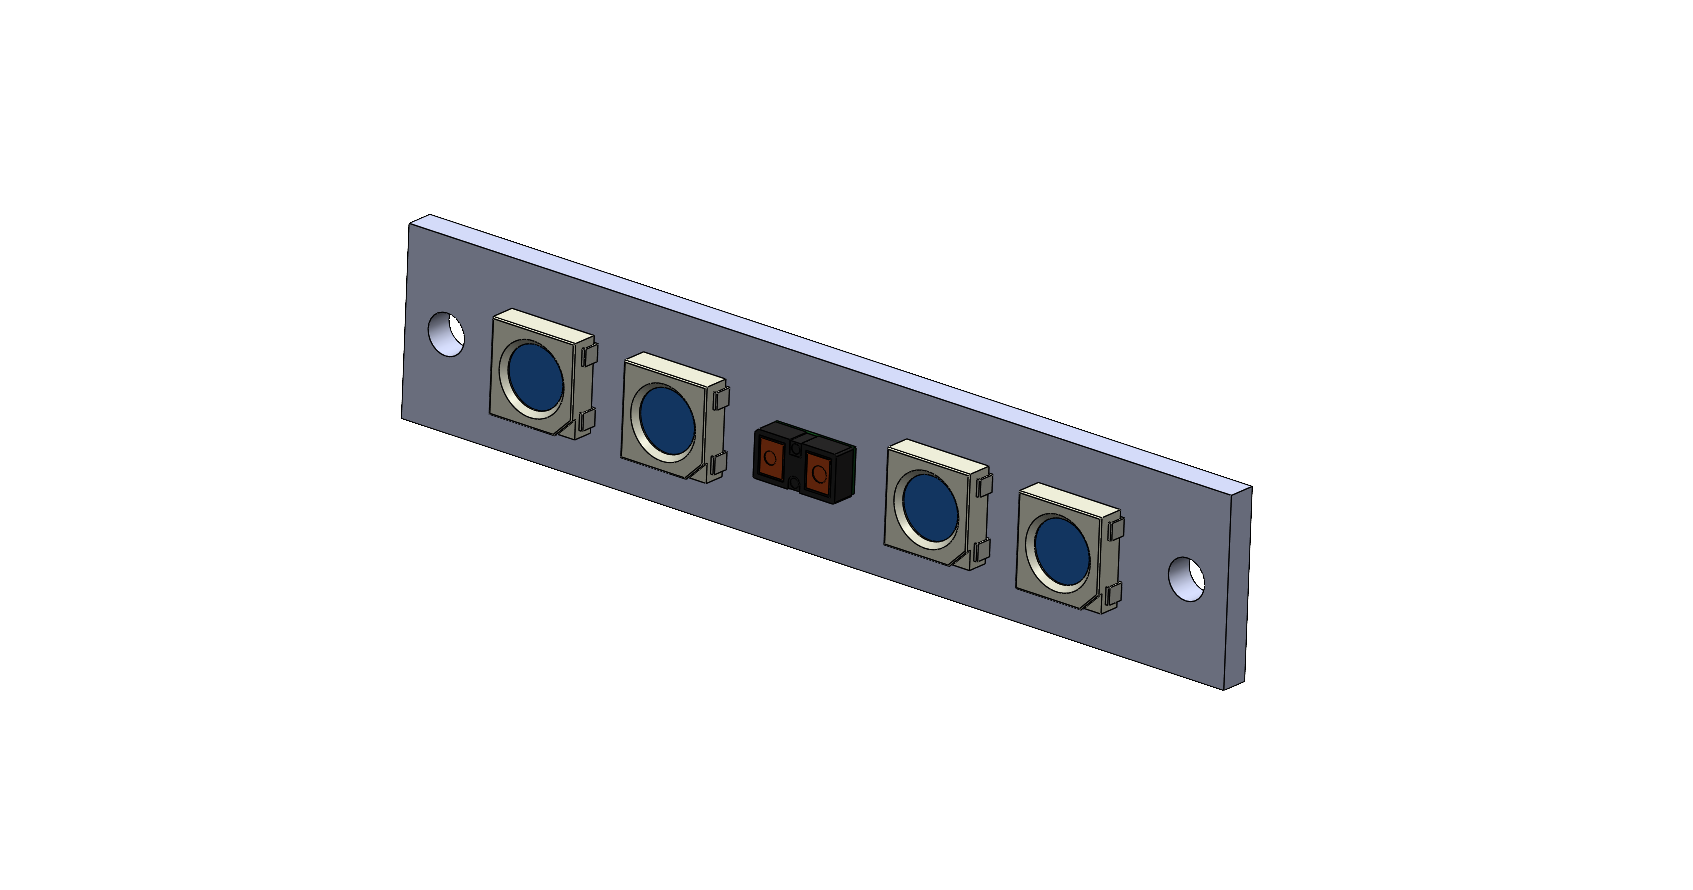
\includegraphics[width=0.5\linewidth]{VL53L1X}
	%\includegraphics[width=0.5\linewidth]{Figures/Mechanical Design/Conceptual_Design}
	\caption[VL53L1X]{VL53L1X}
	\label{fig:VL53L1X}
	\end{figure}
\subsection{Camera}
The Raspberry Pi Camera Module V2 is chosen as a camera for the robot. The camera is chosen because it has a high resolution and it has a high frame rate. The camera has a resolution of 8 MP. The camera has a frame rate of 30 fps. The camera has a maximum current of 250 mA. The camera has a maximum voltage of 3.3 V. The camera has a weight of 3.4 g and a size of 25 x 23 x 9 mm.
%figure of the Raspberry Pi Camera Module V2
\begin{figure}[h]
	\centering
	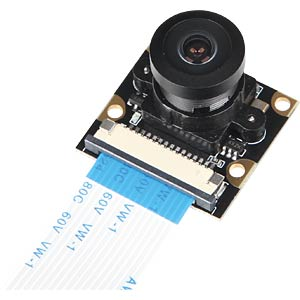
\includegraphics[width=0.5\linewidth]{Raspberry_Pi_Camera_Module_V2}
	%\includegraphics[width=0.5\linewidth]{Figures/Mechanical Design/Conceptual_Design}
	\caption[Raspberry Pi Camera Module V2]{Raspberry Pi Camera Module V2}
	\label{fig:Raspberry_Pi_Camera_Module_V2}
\end{figure}
\newpage
\subsection{Battery}
The SLS XTRON 3000MAH 4S1P 14.8V 35C LIPO BATTERY is chosen as a battery for the robot. The battery is chosen because it has a high capacity and it has a high discharge rate. The battery has a capacity of 3000 mAh. The battery has a discharge rate of 35 C. The battery has a maximum current of 105 A. The battery has a maximum voltage of 16.8 V. The battery has a weight of 300 g and a size of 135 x 42 x 30 mm.
%figure of the SLS XTRON 3000MAH 4S1P
\begin{figure}[h]
	\centering
	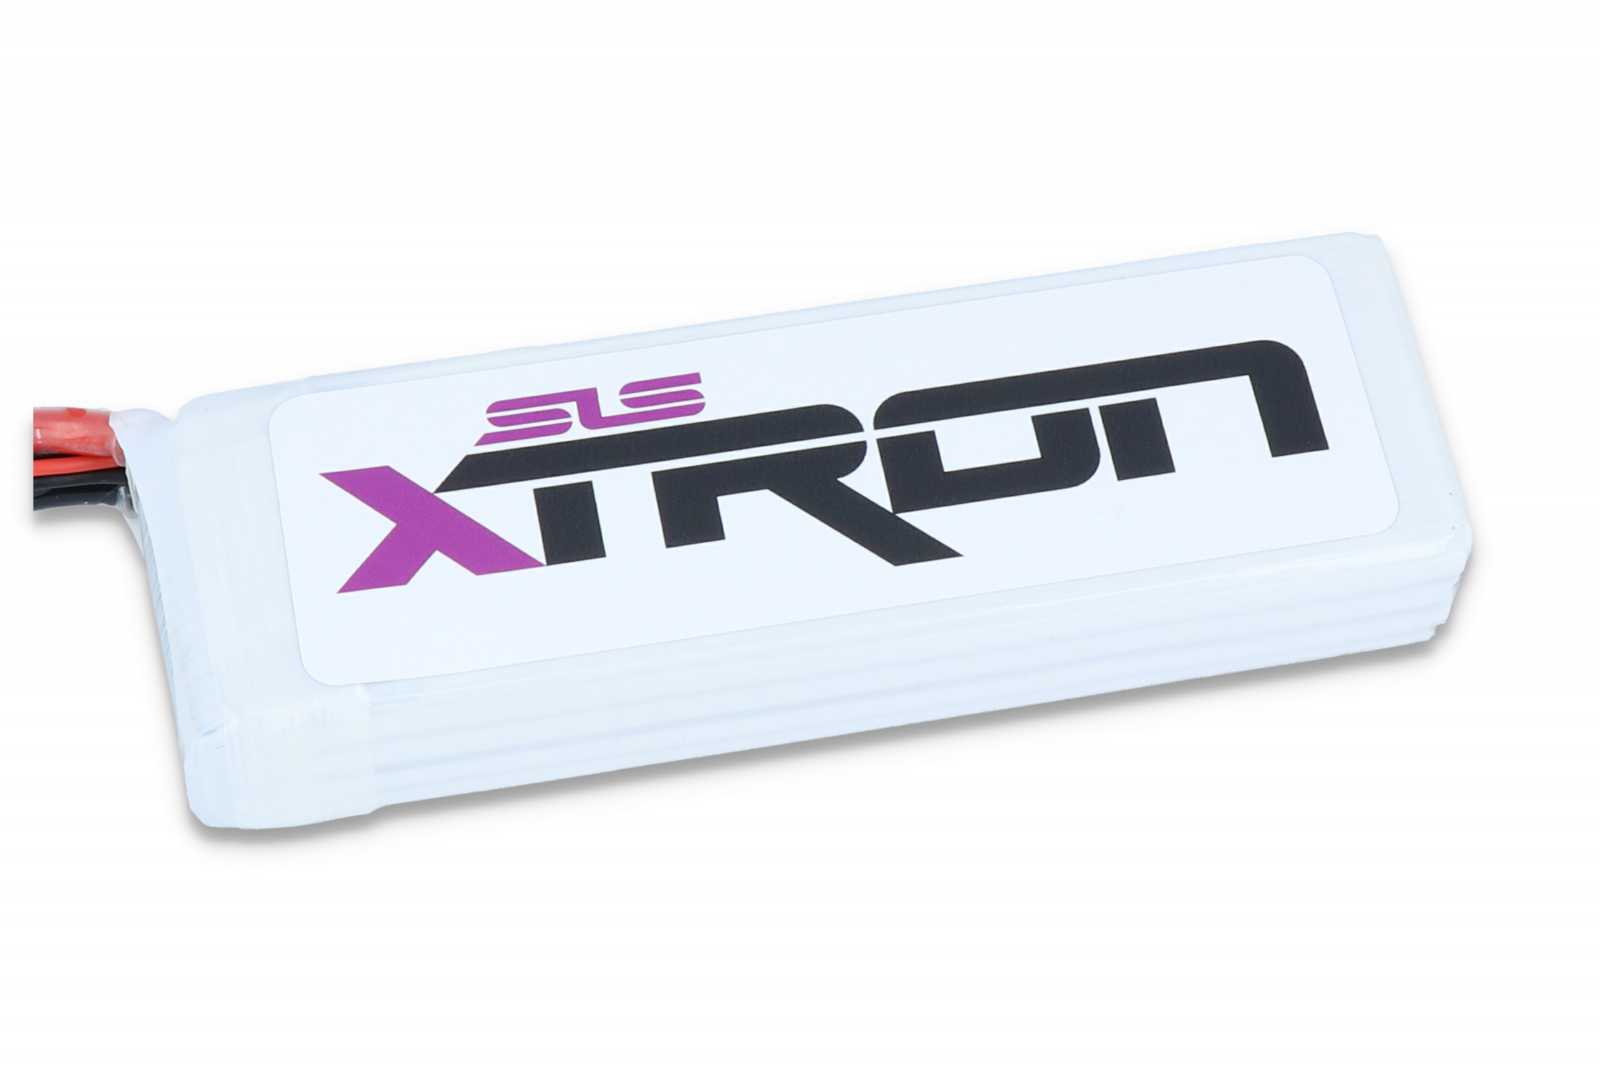
\includegraphics[width=0.5\linewidth]{SLS_XTRON_3000MAH_4S1P}
	%\includegraphics[width=0.5\linewidth]{Figures/Mechanical Design/Conceptual_Design}
	\caption[SLS XTRON 3000MAH 4S1P]{SLS XTRON 3000MAH 4S1P}
	\label{fig:SLS_XTRON_3000MAH_4S1P}
\end{figure}


\section{Circuit Design}
%figure of the electronic design
\begin{figure}[h]
	\centering
	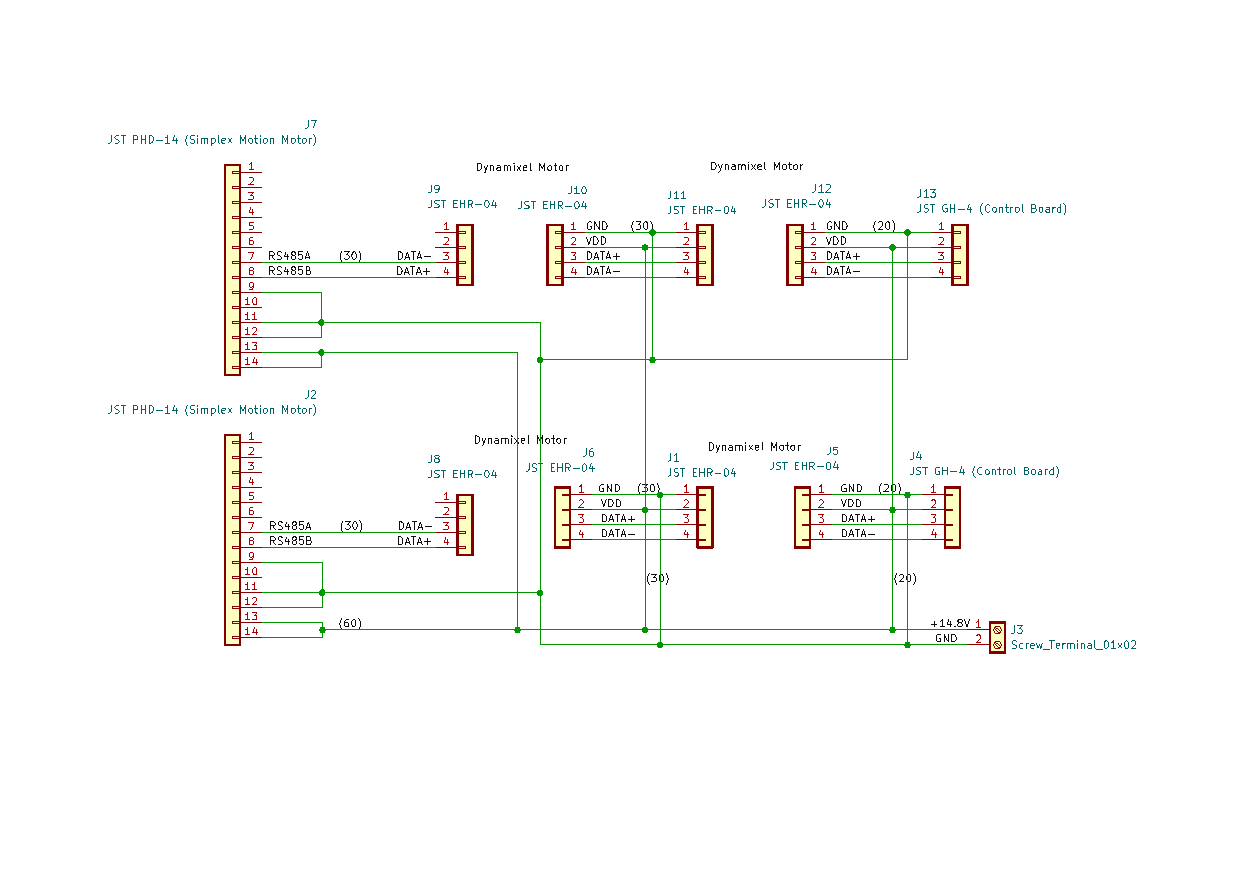
\includegraphics[width=1\linewidth]{Legged_TWIPR_Wiring_Tree}
	%\includegraphics[width=0.5\linewidth]{Figures/Mechanical Design/Conceptual_Design}
	\caption[ brakets for delectronic design second test ]{Electronic Design}
	\label{fig:electronicdesign}
\end{figure}
%expanation of the electronic design
The wiring tree of the electronic components is shown in figure \ref{fig:electronicdesign} where it shows the connection between the different components and the microcontroller.The first motor of each leg is connected to the microcontroller and the rest of the motors are connected in series to the first motor of using daisy chain connection. the motors have the drivers board intigrated so they only need the control signal comimg from the microcontroller. The motor voltage is supplied from the power management board.
%\begin{itemize}
%	\item Provide comprehensive information about the circuit design, including schematic diagrams.
%	\item Explain the functionality and interaction of different circuit components.
%	\item Discuss the design considerations for signal integrity, power distribution, and noise reduction.
%\end{itemize}
\section{Robot Hub Board}
%\subsection{Microcontroller}
%The STM32H7 is chosen as a microcontroller for the robot. The microcontroller is chosen because it has a high processing power and it has a high number of input and output pins. The microcontroller has a 32-bit ARM Cortex-M7 core running at 400 MHz. The microcontroller has 2 MB of flash memory and 1 MB of RAM.
The robot hub board is the main board that connects all the components together.
The board includes the stm32h7 microcontroller that controls the motors and the sensors.
The board also acts as a carrier board for the raspberry pi compute module, where different peripherals can be connected to the raspberry pi via the robot hub board.
High-density edge connector is used to connect the raspberry pi to the robot hub board.
UART is used to communicate between the microcontroller and the raspberry pi.
%figure of the Robot hub board
\begin{figure}[h]
	\centering
	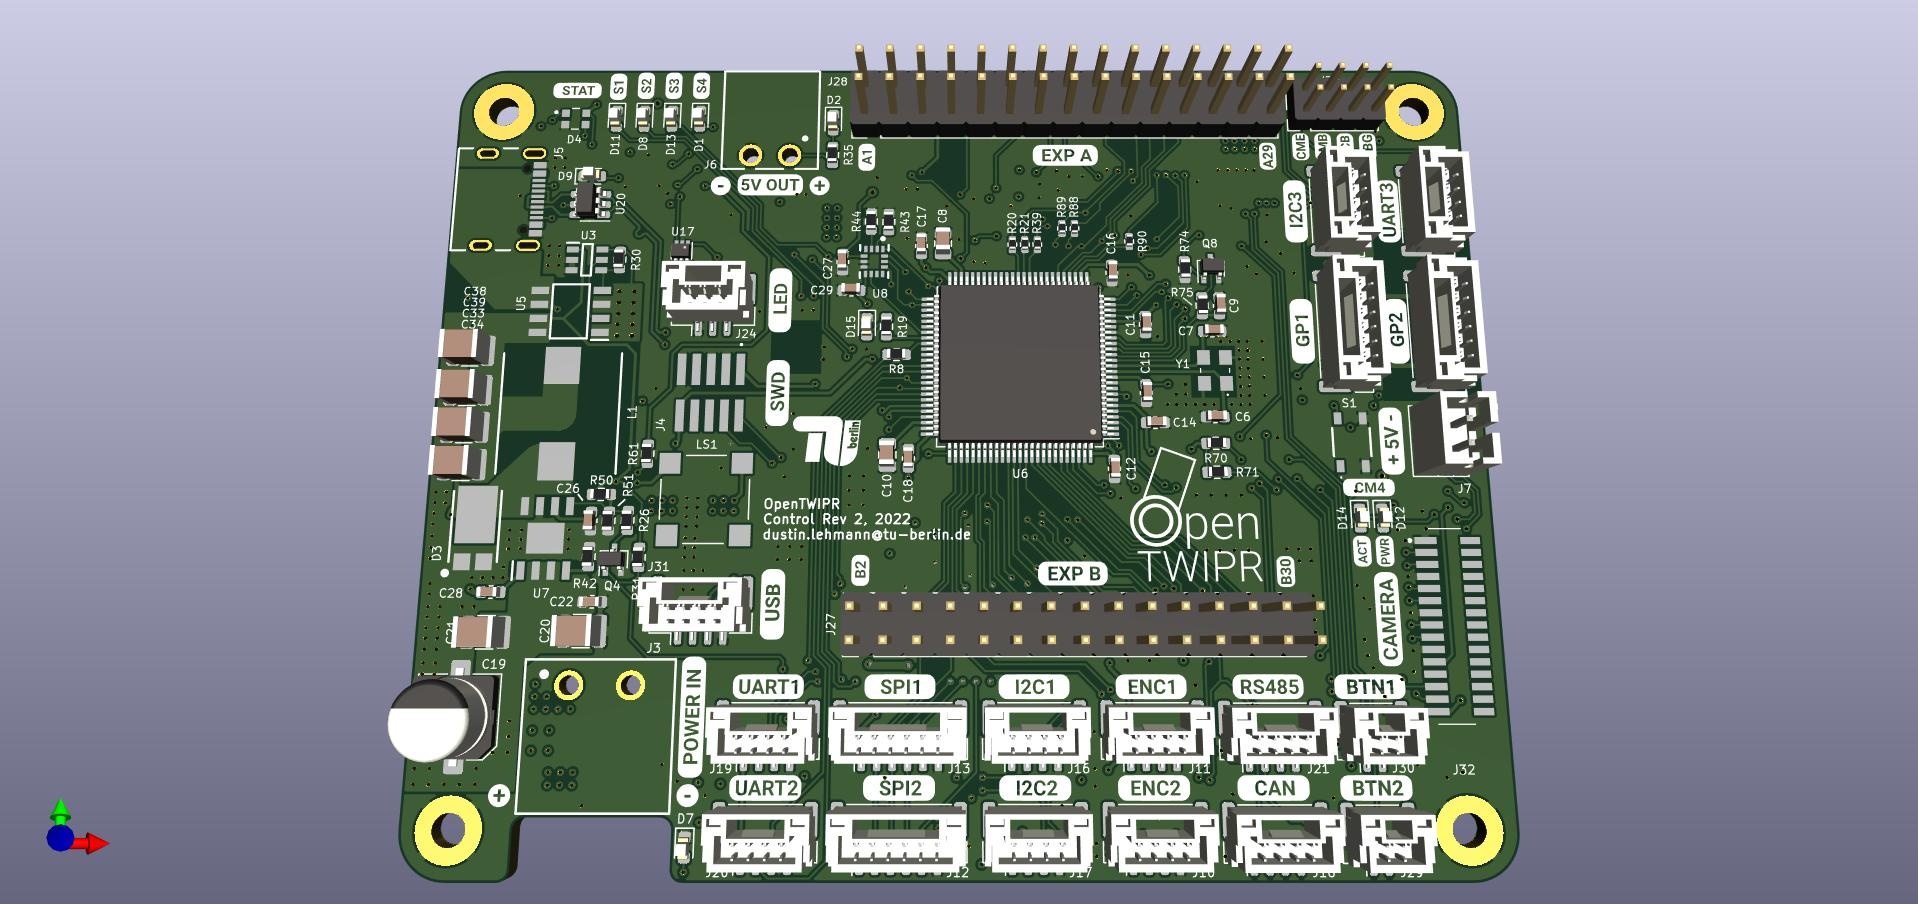
\includegraphics[width=1\linewidth]{Robot_Hub_Board}
	\caption[ Robot Hub Board ]{Robot Hub Board}
	\label{fig:robothubboard}
\end{figure}

%\begin{itemize}
%	\item Describe the layout and design of any custom PCBs used in the project.
%	\item Include information about PCB fabrication and assembly processes.
%\end{itemize}
\newpage
\section{Power Management}
%figure of the power mangment board
\begin{figure}[h]
	\centering
	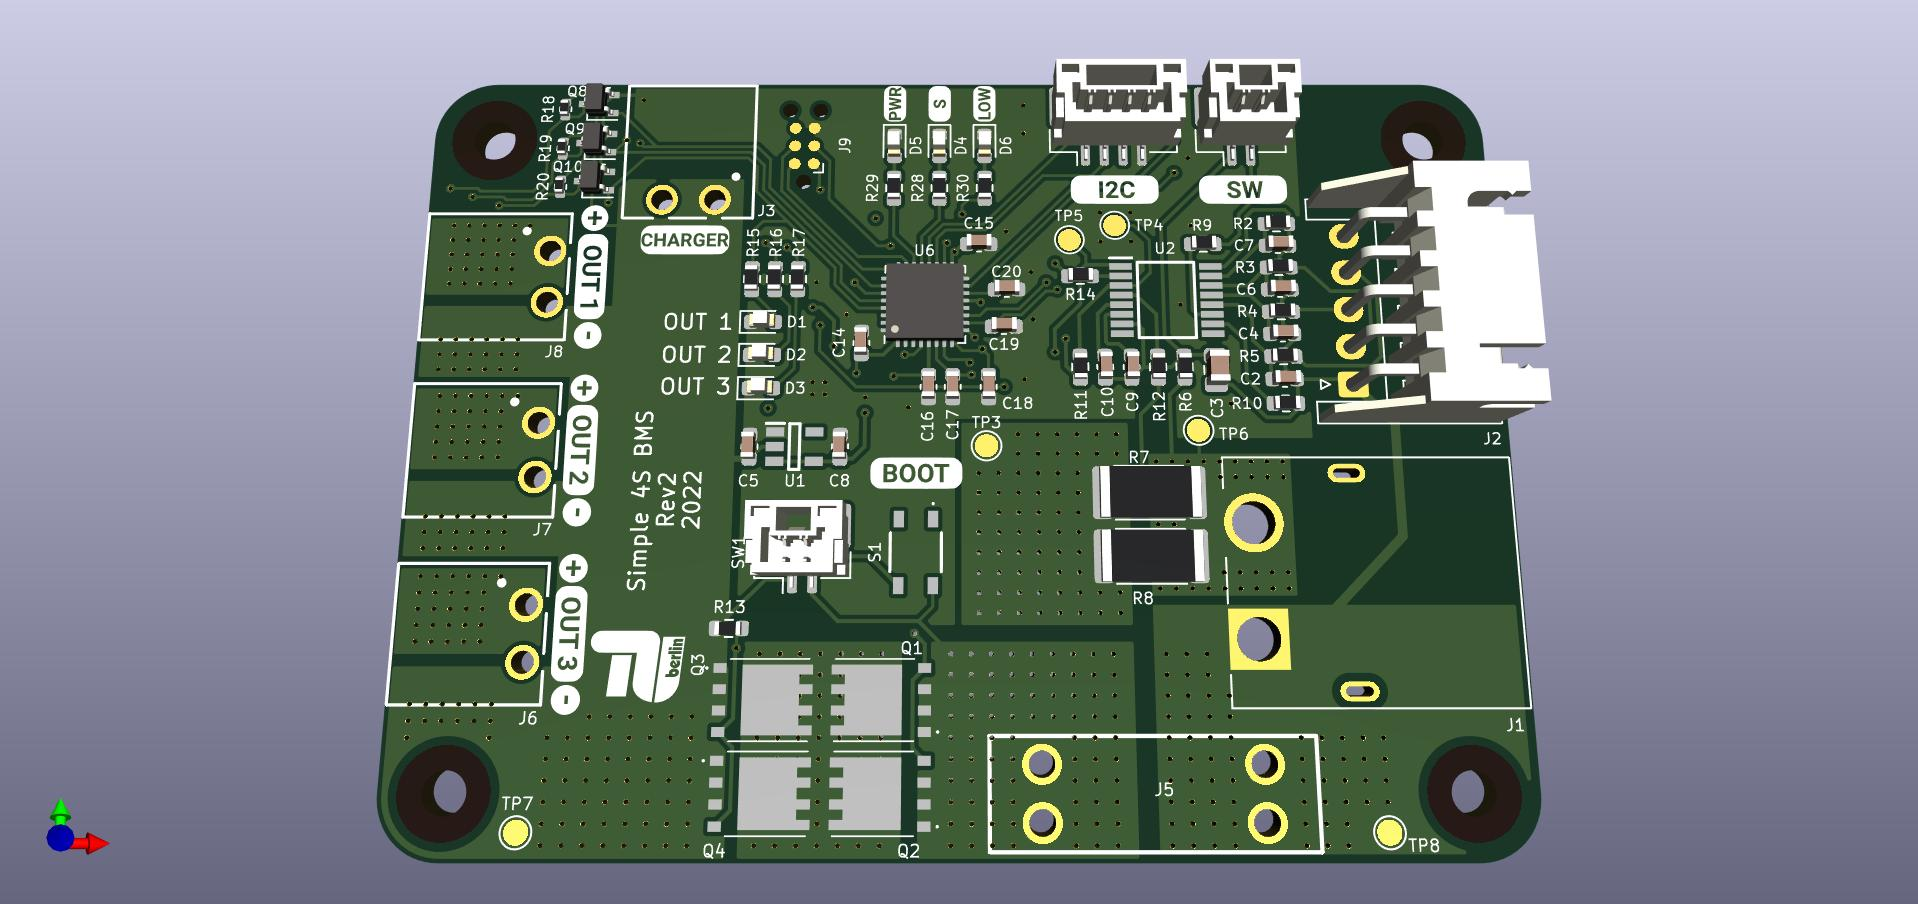
\includegraphics[width=1\linewidth]{Power_Management_Board}
	\caption[ Power Management Board ]{Power Management Board}
	\label{fig:powermanagementboard}
\end{figure}

%For the power management board, can you open the Kicad file for a nice screenshot? If not, I can make one later. But basically it features:
%- 15A Fuse
%- STM32L4 Mikrocontroller for measuring cell voltages and distributing power
%- High Power MOSFET Switches for output power
%- 4-cell battery undervoltage, overvoltage, overcurrent protection
%- Current Measurement
%- Cell Balancing
The power mangment board is responsible for managing the power distribution between the different components. The board has a stm32l4 microcontroller that monitors the battery voltage and the current consumption of the motors. The board has a 15 A fuse that protects the battery from over current. The board has a 4-cell battery undervoltage, overvoltage, overcurrent protection. The board has a cell balancing circuit that balances the voltage between the cells of the battery. The board has a high power MOSFET switches that controls the power distribution between the different components.
%\begin{itemize}
%	\item Discuss how power is managed and distributed within the system.
%	\item Include details on battery management, voltage regulation, and power efficiency considerations.
%\end{itemize}